% !TeX encoding = UTF-8
% !TeX spellcheck = en_GB
% !TeX root = tcas.tex
\documentclass{article}
\usepackage[utf8]{inputenc}
\usepackage{authblk}
\usepackage{setspace}
\usepackage[margin=1.4in]{geometry}
\usepackage{graphicx}
\usepackage{subcaption}
\usepackage{amsmath}
\usepackage{amsthm}
\usepackage{biblatex}
\usepackage{amssymb}
\usepackage{cleveref}
\addbibresource{tcas.bib}

\usepackage{xcolor}
\usepackage{listings}

\definecolor{mGreen}{rgb}{0,0.6,0}
\definecolor{mGray}{rgb}{0.5,0.5,0.5}
\definecolor{mPurple}{rgb}{0.58,0,0.82}
\definecolor{backgroundColour}{rgb}{0.95,0.95,0.92}

\lstdefinestyle{CStyle}{
	backgroundcolor=\color{backgroundColour},   
	commentstyle=\color{mGreen},
	keywordstyle=\color{magenta},
	numberstyle=\tiny\color{mGray},
	stringstyle=\color{mPurple},
	basicstyle=\footnotesize,
	breakatwhitespace=false,         
	breaklines=true,                 
	captionpos=b,                    
	keepspaces=true,                 
	numbers=left,                    
	numbersep=5pt,                  
	showspaces=false,                
	showstringspaces=false,
	showtabs=false,                  
	tabsize=2,
	language=C
}


\title{\textbf{T.C.A.S.}: \textbf{T}CAS \textbf{C}an \textbf{A}lways \textbf{S}olve \\
	\large Numerical Analysis: a Concrete Computational Approach to Limit Evaluation}
\author{Roberto Alessandro Bertolini}

\date{}

\affil{Liceo Nervi Ferrari - Morbegno}
\onehalfspacing

\theoremstyle{plain}
\newtheorem{thm}{Theorem}
\newtheorem*{thm*}{Theorem}

\theoremstyle{definition}
\newtheorem{defn}[thm]{Definition}
\newtheorem*{defn*}{Definition}

\theoremstyle{algorithm}
\newtheorem{algo}{Algorithm}
\newtheorem*{algo*}{Algorithm}

\begin{document}
	\maketitle
	
	\begin{abstract}
		Evaluating limits by hand can become a trivial task with a bit of exercise, but a normal computer is generally incapable of proceeding intuitively and needs a reliable algorithm in order to be able to reach consistently the same result. 
		While some purely heuristic or naive approaches might, at first glance, seem good enough, they tend to quickly fall apart in real world conditions. TCAS is a portable universal C implementation of the Gruntz Algorithm \cite{gruntz}, which at the present day is the most efficient and reliable way of evaluating limits in the exp-log field of operations.
	\end{abstract}
	
	\tableofcontents
	
	\newpage	
	
	\section{Introduction}
	
	\subsection{The Limit of a Function}
	
	The limit of the function $ f: \mathbf{R} \rightarrow \mathbf{R} $ is defined as the following:
	
	\begin{defn*}
		\[ 
		\lim_{x \to x_{0}}{f(x) = l} 
		\]
		
		If and only if \( 
		\forall \varepsilon > 0 \enspace \exists \enspace \delta(\varepsilon) \mid \forall x \in D_{f}, 0 < \mid x - x_{0} \mid < \delta \implies \mid f(x) - l \mid < \varepsilon, \text{where} \: x_{0}, \varepsilon \in \mathbf{R}
		\)
	\end{defn*}
	
	\subsection{Polish Notation} \label{sec:pn}
	
	Jan Lukasiewicz devised the so-called Polish Notation \cite{wiki:polish} in 1924; it is a prefix notation, where the operator precedes its operands.
	As long as the number of operands is predefined, there can't be an ambiguity in the order of evaluation, so this notation doesn't strictly require parenthesis.
	Consider the following expression written without parenthesis:
	
	\[
	8 \times 4 + 3 \times  2 - 6
	\]
	
	Depending on where the parenthesis are placed, it can evaluate to different results:
	
	\[
	(8 \times 4 + 3) \times (2 - 6) = -140; \quad (8 \times (4 + 3) \times 2) - 6 = 106 
	\]
	
	Now consider a similar expression written using polish notation:
	
	\[
	\times \times 8 + 4 \enspace 3 - 2 \enspace 6 = -224
	\]
	
	It necessary evaluates to a single result.
	This makes parsing the expression into an abstract syntax tree \cite{wiki:abtree} much easier, as the parser doesn't have to make educated choices about its interpretation.
	
	\subsection{The Shortcomings of the Naive Approach}
	
	Evaluating a limit might seem easy for a computer, as it should be able to continuously approximate the result with a smaller $\varepsilon$ until the rounding error is acceptable enough, but can this always work?
	Consider the following function:
	
	\[
	f : y = \frac{1}{x^{\ln{\ln{\ln{\ln{\frac{1}{x}}}}}-1}} \tag{1} \label{eq:toinfinity}
	\]
	
	Its graph is the following: \cref{fig:limoff1}, where it seems that for values of x closer to zero the function tends to zero, yet if we compute the limit: \(\lim{x \to 0^{+}}{f(x) = +\infty}\), so the function should have a vertical asymptote in zero. We just can't see it in the graph because it becomes visible for \(x \approx 4.29 \times 10 ^{-1656521}\). A computer trying to approximate the result would have stopped long before this value, returning zero.
	
	What if we try instead to recursively apply L'Hôpital's rule \cite{wiki:hopital} until we reach a clear result?
	Consider the following functions:
	
	\[
	f(x) = e^{x} + e^{-x}
	\] 
	\[
	g(x) = e^{x} - e^{-x}
	\]
	
	\[
	\lim_{x \to \infty}{\frac{f(x)}{g(x)}} = \lim_{x \to \infty}{\frac{f''(x)}{g''(x)}} = \lim_{x \to \infty}{\frac{e^{x} + e^{-x}}{e^{x} - e^{-x}}}
	\]
	
	So recursively applying L'Hôpital's rule would not work in this case.
	
	\section{The Gruntz Algorithm}
	
	\subsection{Manipulating the Most Rapidly Varying Subexpressions}
	
	\begin{defn*}
		\(g(x)\) is said to be a subexpression of \(f(x)\) if the evaluation of \(f(x)\) causes the evaluation of \(g(x)\). This is represented with the following notation:
		\[
		\begin{aligned}
			g(x) \triangleleft f(x)&\text{, if} \: g(x) \: \text{is a subexpression of} \: f(x) \\
			g(x) \ntriangleleft f(x)&\text{, if} \: g(x) \: \text{is not a subexpression of} \: f(x)
		\end{aligned}
		\]
	\end{defn*}
	
	\begin{defn*}
		Two subexpressions \(g(x)\) and \(h(x)\) can be compared based on their comparability class, which describes how rapidly they vary.
		\[
		\begin{aligned}
			f(x) \prec g(x) \: \text{if and only if} \enspace &\lim_{x \to \infty}{\frac{\ln{\mid f(x)\mid}}{\ln{\mid g(x)\mid}}} = 0 \\ 
			f(x) \asymp g(x) \: \text{if and only if} \enspace &\lim_{x \to \infty}{\frac{\ln{\mid f(x)\mid}}{\ln{\mid g(x)\mid}}} \neq 0 \in \mathbf{R}
		\end{aligned} \tag{2}
		\] \label{defn:comparability}
	\end{defn*} 
	
	\begin{defn*}
		The MRV set is the set that contains all the subexpressions of the highest comparability class.
		\[
		mrv(f(x)) = \begin{cases}
			\{\} \quad \text{if} \enspace x \ntriangleleft f(x) \\
			\{g(x) \mid g(x) \triangleleft f(x) \wedge (\nexists \enspace h(x) \triangleleft f(x) \mid h(x) \succ g(x)))\}
		\end{cases}
		\]
	\end{defn*} \label{defn:mrv}
	
	The first step of the Gruntz algorithm is recursively computing the MRV set of the limit that needs evaluating. If empty, the limit is indipendent of x. 
	Once found, all the subexpressions contained in it must be rewritten as a function of \(w\), which itself has to respect the following expression: 
	\[
	\lim_{x \to \infty}{w(x)} = 0+
	\]
	The most common \(w\) is \(w(x) = e^{-x}\).
	
	\subsection{Power Series Representation}
	
	\begin{defn*}
		The Maclaurin series of any function is defined as the following:
		\[
		\sum_{n=0}^{\infty}{\frac{f^{(n)}(0)}{n!} x^{n}}
		\]
	\end{defn*}
	
	For the algorithm we need the first non-zero term of the Maclaurin series of the function after the \(w\) substitution, which will be in the form \(A(x)w^b\).
	
	The final result of the limit will be the following:
	
	\[
	\lim_{x \to x_{0}}{f(x)} = \lim_{x \to 0}{w(x)} = \begin{cases}
		0 &\text{if} \: b > 0 \\
		+\infty &\text{if} \: b < 0\\
		\lim_{x \to 0}{A(x)} &\text{if} \: b = 0
	\end{cases}
	\]
	
	\subsection{Caveats and Limitations}
	
	The Gruntz algorithm, while mathematically proven to be always valid in the exp-log field of operations, has some caveats that, if not handled correctly, might prevent it from reaching the correct result, or reaching a result at all. Firstly, before computing the MRV, the limit has to be rewritten so that it tends to \(+\infty\), applying some smart substitutions.
	Computing the correct MRV set is a complex operation, which involves recursively evaluating limits, which are proven to be of lower complexities only if simplifications are applied all throughout the process. If the MRV is of a lower comparability class compared to \({x}\), the limit has to be rewritten so that the MRV increases its comparability class, usually applying the following definition:
	
	\begin{defn*}
		\[
		\lim_{x \to +\infty}{f(x)}=+\infty \: \bigwedge \: \lim_{x \to +\infty}{g(x)}=+\infty \implies \lim_{x \to +\infty}{f(g(x))}=+\infty
		\]
	\end{defn*}
	
	\section{T.C.A.S.}
	
	\subsection{Parsing the Expression}
	
	The first thing that TCAS does is parsing the input string. The space-separated chain of operators and operands needs to be interpreted as a concrete syntax tree \cite{wiki:parsetree}\cite{wiki:abtree}, where every operator is a branch node and every symbol or value is a leaf node; this happens in multiple step.\\
	Firstly, the input string is tokenized, so it is split into an array of tokens based on a common delimiter which is the space character; this happens in linear time \(O(n)\). \\
	This array of tokens goes through the Polish Notation [\ref{sec:pn}] interpreter, which in linear time \(O(n)\) builds a concrete syntax tree, branching when the token is recognized to be an operator and terminating with a leaf for anything else. \\
	This tree is incomplete though, as symbols and values are still in their string representation and have yet to be parsed; this happens in the translator, which, again in linear time \(O(n)\) loops once over the concrete syntax tree and replaces every node with an \textit{expr\_tree\_link}, \cref{fig:expr_structs}, \cref{code:expr_structs}; see \cref{fig:parser} for a representation of the whole process.
	
	\subsection{Finding the MRV}
	
	Finding the MRV is a complex operation which involves multiple steps. 
	The root node, which should always have branches, goes through \textit{\_mrv\_op}, \cref{code:mrv_op}. Dominikiz Gruntz provided a pseudo-code representation of what \textit{\_mrv\_op} should do, which has been slightly altered here so that the method names correspond to their implementation:
	
	\begin{algo*}
		Computing the MRV set of \(f\) \\
		\[
		\begin{aligned}
			\text{mrv}\:&(f : \text{exp-log function in} \: x) \\
			&\begin{aligned}
				&\text{if} &x \ntriangleleft f & \rightarrow RETURN(\:\{\}\:) \\
				&\text{elif} &f = x & \rightarrow RETURN(\:\{x\}\:) \\
				&\text{elif} &f = g \times h & \rightarrow RETURN(\:\{\text{\_mrv\_max}(\text{\_mrv\_generic}(g), \text{\_mrv\_generic}(h))\}\:) \\
				&\text{elif} &f = g + h & \rightarrow RETURN(\:\{\text{\_mrv\_max}(\text{\_mrv\_generic}(g), \text{\_mrv\_generic}(h))\}\:) \\
				&\text{elif} &f = g^{c} \wedge c \in \mathbf{R} & \rightarrow RETURN(\:\{\text{\_mrv\_generic}(g)\}\:) \\
				&\text{elif} &f = \ln{c} & \rightarrow RETURN(\:\{\text{\_mrv\_generic}(g)\}\:) \\
				&\text{elif} &f = g^{c} & \rightarrow RETURN(\:\{\text{\_mrv\_exp}(g)\}\:) \\
				&\text{fi}
			\end{aligned}
		\end{aligned}
		\]
	\end{algo*}

	The method \textit{\_mrv\_max} makes use of the definition in \eqref{defn:comparability}, with some common options coded in for performance optimization purposes; \textit{\_mrv\_generic} is an internal reference to \textit{mrv}; \textit{\_mrv\_exp} is a special function that handles the MRV  of exponential functions: for the generic form \(e^{g}\), if \(\lim_{x \to +\infty}{g} = \pm\) then the MRV is \textit{\_mrv\_max(\{\(e^{g}\)\}, \_mrv\_generic(g))}, else \(g \succ e^{g}\) so the MRV is \(\_mrv\_generic(g)\).
	
	\subsection{Evaluating the Result}
	
	
	
	\subsection{Performance Considerations}
	
	C was chosen as the programming language for multiple reasons: it is portable, it is universal, it is fast and it is easy to use.
	The most commonly used implementation of the Gruntz algorithm is in SymPy \cite{10.7717/peerj-cs.103}, a Python library for symbolic mathematics. \\
	There are almost no similarities between C and Python \cite{book:python}, with the former being a statically-typed \cite{wiki:typesystem} compiled language and the latter being a dynamically-typed \cite{wiki:typesystem} interpreted one. 
	Multiple tests were run on both implementations, with the results showing an interesting pattern: \cref{fig:performance_graph}. After "warming up" SymPy, so that it loads all the dynamically-linked libraries and extensions, which was done by making it evaluate the simple limit \(\lim_{x \to 0}{\frac{\sin(x)}{x}}\), the running time seems to scale linearly between the two systems in the first three tests. The difference is most probably due to the fact that SymPy runs in an interpreted language, so every instruction has to be parsed, evaluated and executed, while TCAS is compiled to machine code is directly and just executed. \\
	Test-4 shows an advantage that SymPy has over TCAS: its ability to cache frequent operations; this feature, which is mostly trivial to implement, isn't ready yet, so on longer, repeated operations SymPy is able to reuse the old result and skip all the processing. This feature has some side-effects that must be considered: an increased memory usage, a small but perceivable performance reduction if the result has never been cached before, an increased complexity in memory management; if ever implemented, it should remain an opt-out feature for the cases when it might not be beneficial, \textit{e.g.} on microcontrollers for PID \cite{wiki:pid} feedback mechanisms.
	Additional considerations could be made by \textit{ptracing} \cite{wiki:ptrace} both executables.
	
	
	\newpage
	\nocite{book:kr}
	\nocite{pdf:gnump}
	\nocite{pdf:mpfr}
	\printbibliography
	
	\newpage
	\appendix
	\begin{figure}
		\centering
		\includegraphics[width=0.9\textwidth]{img/limoff1.PNG}
		\caption{The graph of \eqref{eq:toinfinity}}\label{fig:limoff1}
	\end{figure}

	\begin{figure}
		\centering
		\includegraphics[width=0.9\textwidth]{chart/expr_structs.PNG}
		\caption{The entity representation of a generic node, with color-coded combinations} \label{fig:expr_structs}
	\end{figure}

	\begin{figure}
		\centering
		\includegraphics[width=0.7\textwidth]{chart/parser.PNG}
		\caption{A short flowchart of how the parser works} \label{fig:parser}
	\end{figure}

	\begin{figure}
		\centering
		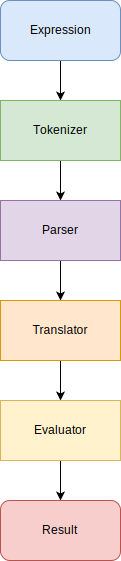
\includegraphics[width=0.7\textwidth]{chart/general_flowchart.PNG}
		\caption{A short flowchart of how TCAS works} \label{fig:tcas} 
	\end{figure}

    \begin{figure}
		\centering
		\includegraphics[width=0.7\textwidth]{img/performance_graph.PNG}
		\caption{The graph is a performance comparison between TCAS and SymPy in four different tests.\\SymPy was "warmed up" prior to the test.\\Test-1 evaluated 200 times the same limit.\\Test-2 evaluated the same 3 limits for 100 times.\\Test-3 evaluated a very complex nested limit.\\Test-4 re-ran Test-1 for 10 times} \label{fig:performance_graph}  
	\end{figure}

	\begin{figure}
	\centering
	\begin{lstlisting}[style=CStyle]
		#ifndef EXPR_STRUCTS_H
		#define EXPR_STRUCTS_H
		
		#include <stdio.h>
		#include <stddef.h>
		#include <gmp.h>
		#include <mpfr.h>
		
		enum VAL_TYPE {
			INT = 0b001,
			RATIONAL = 0b010,
			FLOAT = 0b100,
		};
		
		struct expr_tree_head {
			struct expr_tree_link *head;
		};
		
		struct expr_tree_op {
			enum OPERATOR_TYPE type;
			size_t arg_count;
			struct expr_tree_link **args;
		};
		
		struct expr_tree_val {
			enum VAL_TYPE type;
			union expr_tree_val_ref *val;
		};
		
		struct expr_tree_sym {
			char sign;
			char representation;
		};
		
		struct expr_tree_link {
			enum LINKED_TYPE type;
			union expr_tree_ptr *ptr;
		};
		
		union expr_tree_ptr {
			struct expr_tree_val *val;
			struct expr_tree_op *op;
			struct expr_tree_sym *sym;
		};
		
		union expr_tree_val_ref {
			mpz_t int_val;
			mpq_t rational_val;
			mpfr_t fp_val;
		};
		
		
		#endif
		
	\end{lstlisting}
	\caption{The code that defines the concrete syntax tree} \label{code:expr_structs}
\end{figure}

\begin{figure}
	\centering
	\begin{lstlisting}[style=CStyle]
		struct ps_leadterm {
			int term_num;
			struct expr_tree_link *coeff;
			struct expr_tree_val *exp;
		};
	\end{lstlisting}
	\caption{How the first term of the power series is represented} \label{code:ps_structs}
\end{figure}

\begin{figure}
	\centering
	\begin{lstlisting}[style=CStyle]
		struct expr_tree_link *compute_gruntz_result(struct expr_tree_link *link) {
			struct ps_leadterm *term = _recursive_compute_lt(link);
			
			while (term->exp->type != INT) {
				term = _recursive_lt_next(term, link);
			}
		
			if (mpz_cmp_si(term->exp->val->int_val, 0) > 0) {
				return parse_expr("+infinity", NULL);
			} else if (mpz_cmp_si(term->exp->val->int_val, 0) == 0) {
				return gruntz_eval(term->coeff);
			} else {
				return parse_expr("0", NULL);
			}
		}
	\end{lstlisting}
	\caption{How the result is evaluated} \label{code:ps_result}
\end{figure}

\begin{figure}
	\centering
	\begin{lstlisting}[style=CStyle]
		struct gruntz_mrv {
			size_t count;
			struct gruntz_expr **expr;
		};
		
		struct gruntz_expr {
			struct expr_tree_link *expr;
		};
	\end{lstlisting}
	\caption{How the MRV structs are defined} \label{code:mrv_structs}
\end{figure}

\begin{figure}
	\centering
	\begin{lstlisting}[style=CStyle]
		struct gruntz_mrv *_mrv_op(struct expr_tree_link *link) {
			switch (link->ptr->op->type) {
				case PLUS:
				case MINUS:
				case TIMES:
				case DIVIDE:
					return _mrv_max(_mrv_generic(link->ptr->op->args[0]), _mrv_generic(link->ptr->op->args[1]));
				case SQRT:
				case SIN:
				case COS:
				case TAN:
				case LN:
				case LOG10:
				case LOG2:
					return _mrv_generic(link->ptr->op->args[0]);
				case ROOT:
				case POWER:
					assert(link->ptr->op->args[1]->type == VALUE);
					return _mrv_generic(link->ptr->op->args[0]);
				case EXP:
					return _mrv_exp(link);
				default:
					assert(0);
			}
		}
	\end{lstlisting}
	\caption{\textit{\_mrv\_op}, refer to \cref{code:expr_structs} and \cref{code:mrv_structs} for how the data types are implemented} \label{code:mrv_op}
\end{figure}
	
\end{document}
